\chapter{\en{Containerization} και \en{Deployment} }

\section{\en{Containerization} με \en{Docker}}

\subsection{Δημιουργία \en{Docker Image}}

Προκειμένου να μπορέσουμε να χρησιμοποιήσουμε το \en{Docker Desktop}, θα πρέπει να έχουμε δημιουργήσει την εφαρμογή μας σε μορφή \en{container}. Για να το πετύχουμε αυτό, είναι απαραίτητο να δημιουργήσουμε το \en{Dockerfile}(Σχήμα 8.1), το οποίο ουσιαστικά μετατρέπει την εφαρμογή μας σε \en{container}.
Προτού εξηγήσουμε τη διαδικασία δημιουργίας του \en{Image}, είναι σημαντικό να αναφέρουμε τον λόγο για τον οποίο πραγματοποιείται αυτή η διαδικασία. Οι \en{Cloud Native microservices} είναι σχεδιασμένες να λειτουργούν πάνω στην υποδομή του \en{Kubernetes}. Για να μπορέσει το \en{Kubernetes} να τις διαχειριστεί, πρέπει να γίνουν \en{deploy} σε αυτόν.
Ο \en{Kubernetes} δεν αναγνωρίζει εφαρμογές, ούτε \en{containers}, ούτε \en{Images} αλλά μόνο \en{pods}. Τα \en{pods} περιέχουν τα \en{containers}, τα οποία ουσιαστικά αποτελούν το λογισμικό που δημιουργείται μέσω της διαδικασίας δημιουργίας του \en{Image}. Ο Κυβερνήτης δεν αναγνωρίζει τίποτα άλλο εκτός από τα \en{pods}. Επειδή, λοιπόν, ο \en{Kubernetes} αναγνωρίζει \en{pods} που ορίζονται μέσω αρχείων \en{YAML}, τα οποία αναλύονται εκτενέστερα στην παράγραφο 8.2.1, δημιουργούμε το \en{Image} με τέτοιο τρόπο ώστε να μπορεί να το αναγνωρίσει ο \en{Kubernetes} στο τοπικό \en{Docker repository} και να προχωρήσει στη δημιουργία του \en{pod}.


\begin{figure}[htb]
	\centering
	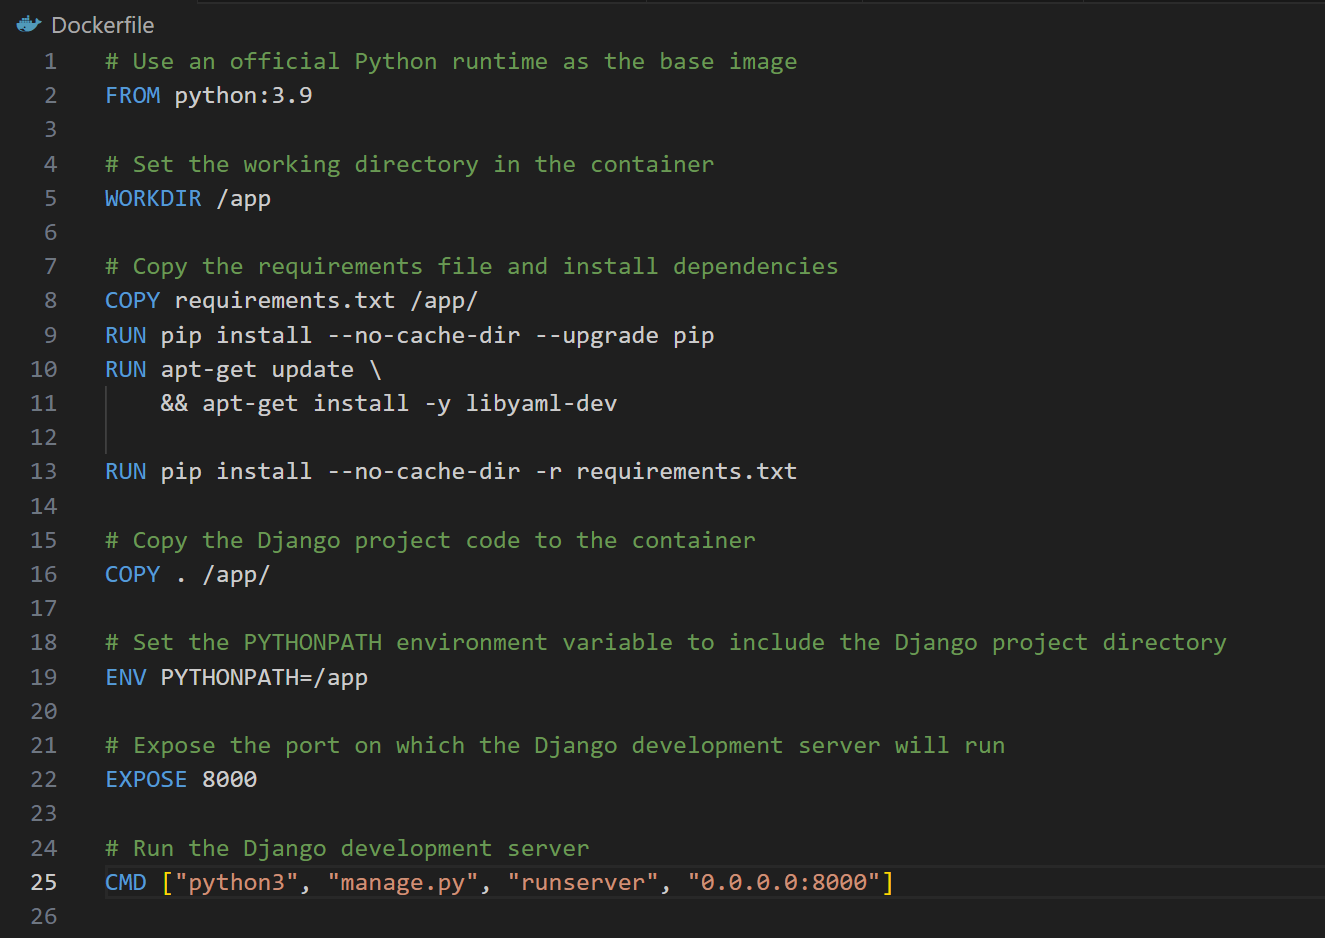
\includegraphics[width=1.5\textwidth]{graphics/dockerfile.png}
	\caption{\en{Dockerfile}}
\end{figure}

\FloatBarrier


Tο \en{Dockerfile} του σχήματος 8.1 δηµιουργεί ένα περιβάλλον \en{Python 3.9} για ένα έργο \en{Django}. Ορίζει το φάκελο εργασίας στον κατάλογο \en{/app}, εγκαθιστά τις απαιτούµενες εξαρτήσεις από το αρχείο \en{requirements.txt}(σχήμα 8.4) , ενηµερώνει το \en{pip}, και εγκαθιστά βιβλιοθήκες συστήµατος (π.χ. \en{libyaml-dev}). Αντιγράφει τον κώδικα του έργου \en{Django} στο κοντέινερ, θέτει τη µεταβλητή περιβάλλοντος \en{PYTHONPATH}, εκθέτει την θύρα 8000 για τον διακοµιστή \en{Django} και εκκινεί την εφαρµογή µε την εντολή \en{runserver}.


Η εντολή \en{docker build}(σχήμα 8.2) χρησιμοποιείται για τη δημιουργία μιας εικόνας \en{Docker} (\en{Docker image}) 
από ένα συγκεκριμένο αρχείο \en{Dockerfile} και τα αρχεία που περιλαμβάνονται στον φάκελο εργασίας (\en{context}).

Αυτή η διαδικασία πακετάρει τον κώδικα της εφαρμογής, τις εξαρτήσεις και τις ρυθμίσεις σε ένα απομονωμένο περιβάλλον. 
Με αυτόν τον τρόπο, η παραγόμενη εικόνα μπορεί να διαμοιραστεί και να εκτελεστεί με συνέπεια σε διαφορετικά συστήματα, 
εξασφαλίζοντας ομοιόμορφο περιβάλλον εκτέλεσης. Είναι σημαντικό εργαλείο για αυτοματοποίηση και ανάπτυξη σε συστήματα \en{CI/CD}. Για να φτιάξουμε το \en{image} τρέχουμε τη εντολη \en{docker build -t djangothesis:v2}(σχήμα 8.2). Για να μπορέσουμε να τρέξουμε την εντολή αυτή πρέπει να βρισκόμαστε στο \en{path} που βρίσκεται το \en{requirements.txt} και το \en{manage.py}. Η διαδρομή φαίνεται στο σχήμα 8.3. 

\FloatBarrier

\begin{figure}[h]
	\centering
	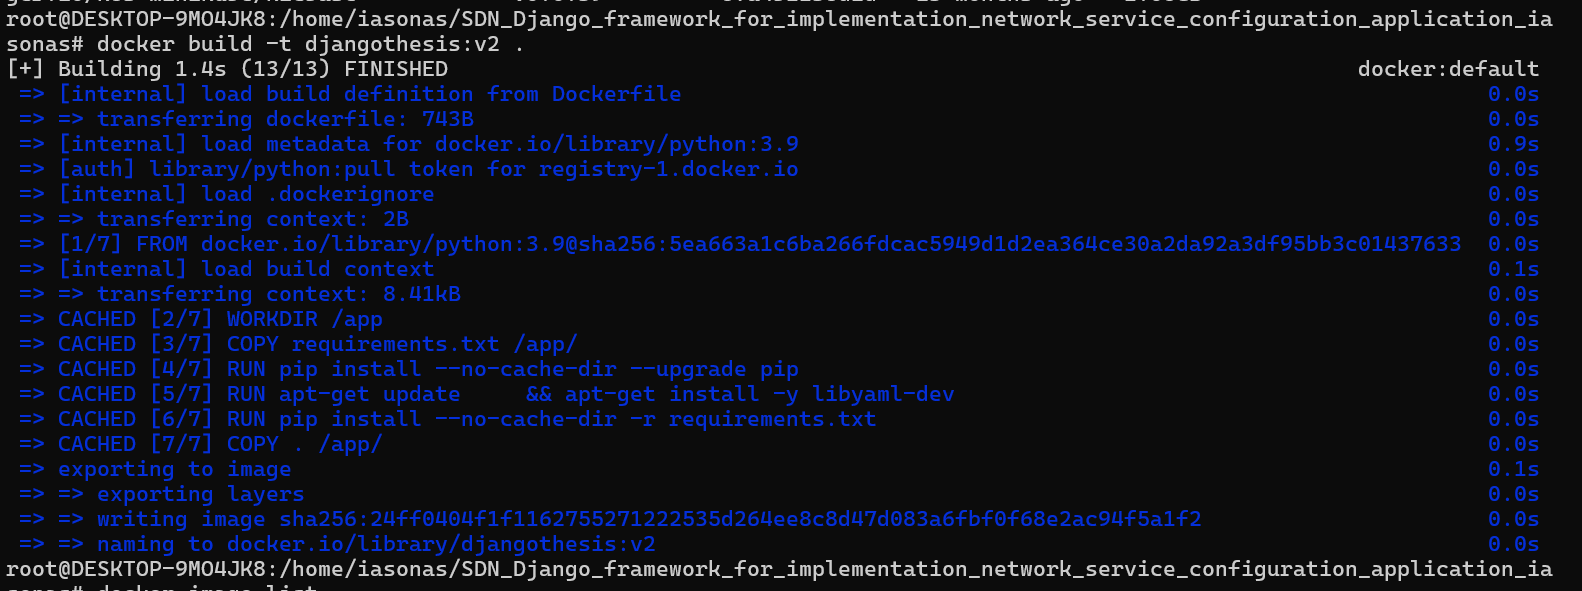
\includegraphics[width=1.0\textwidth]{graphics/docker_build_v2.png}
	\caption{\en{Docker build}-Δημιουργία του κοντεινερ}
\end{figure}

\FloatBarrier


\FloatBarrier

\begin{figure}[h]
	\centering
	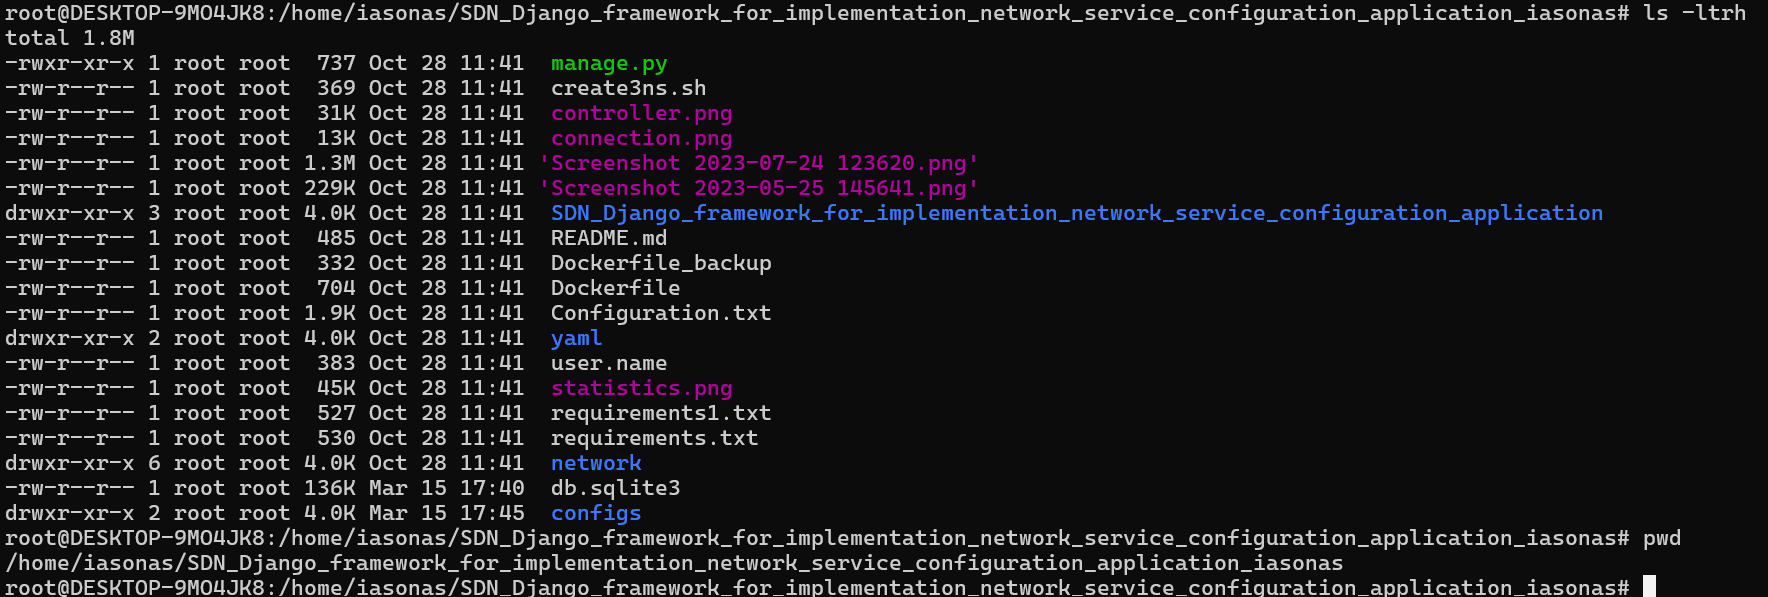
\includegraphics[width=1.0\textwidth]{graphics/dockerfile_location.png}
	\caption{\en{Dockerfile Path}}
\end{figure}

\FloatBarrier

\FloatBarrier

\begin{figure}[h]
	\centering
	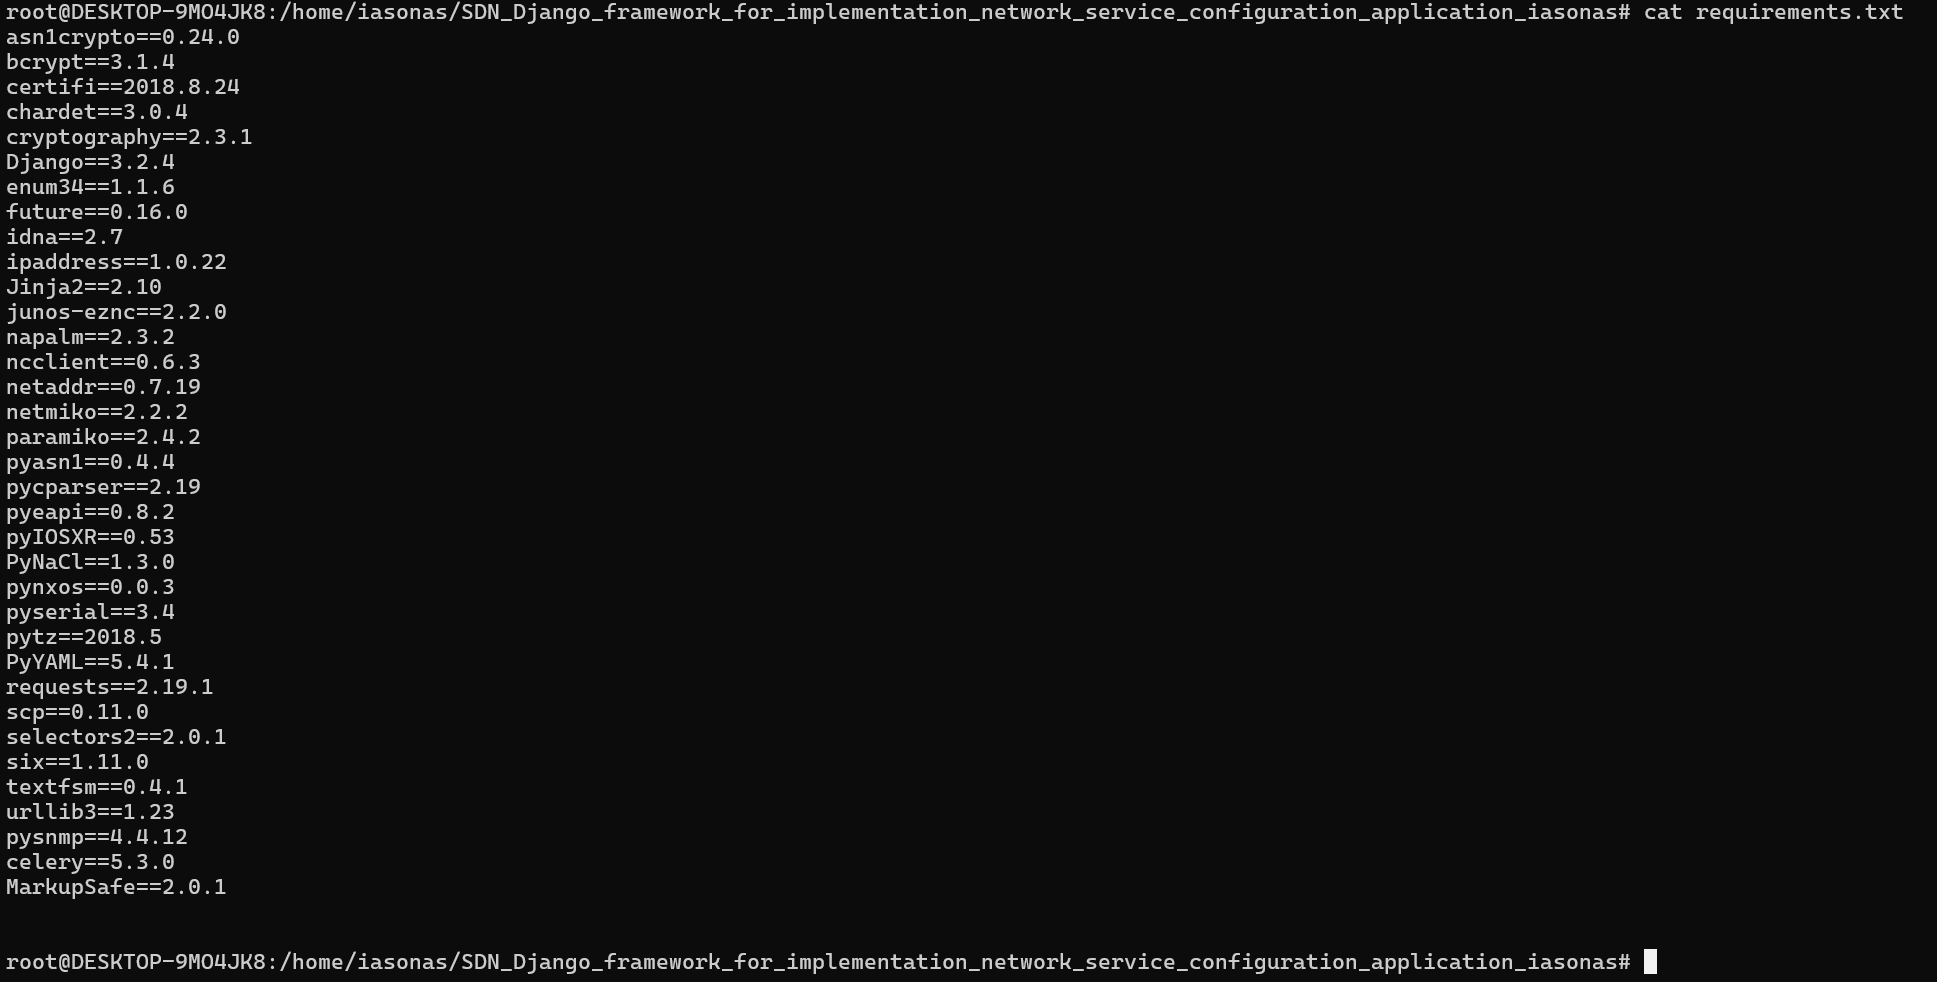
\includegraphics[width=1.0\textwidth]{graphics/requirements.png}
	\caption{\en{requirements.txt}}
\end{figure}

\FloatBarrier

\noindent Τώρα που έγινε \en{build} το \en{image} είναι διαθέσιμο τοπικά(σχήμα 8.5) με το όνομα \en{djangothesis} και \en{tag v2} όπως αυτό ορίστηκε από την εντολή \en{docker build}(σχήμα 8.2).

\FloatBarrier


\begin{figure}[h]
	\centering
	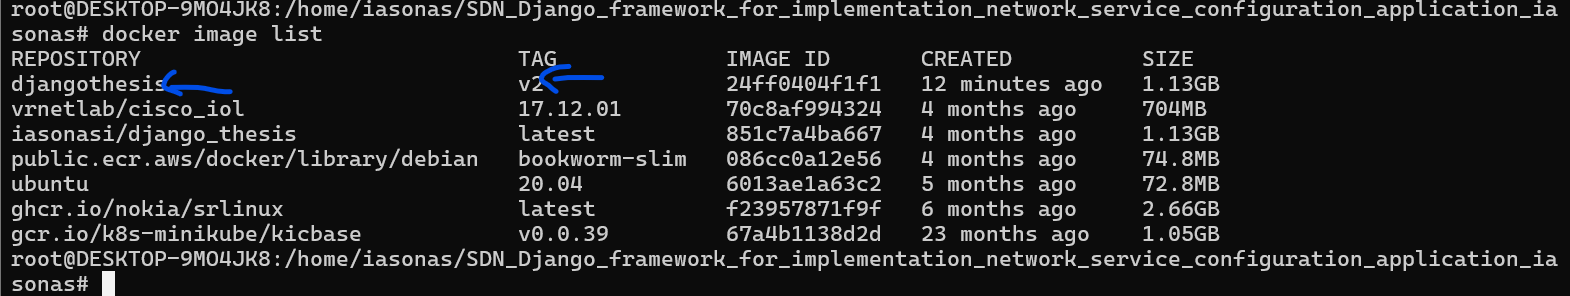
\includegraphics[width=1.5\textwidth]{graphics/docker_image_list_2.png}
	\caption{\en{Docker image list}}
\end{figure}

\FloatBarrier



\section{\en{Deployment} με \en{Kubernetes}}

Τα τελευταία χρόνια, παρατηρείται ραγδαία αύξηση στον τομέα της πληροφορικής, 
με την εμφάνιση και εξάπλωση νέων εννοιών, όπως ο κυβερνήτης και τα \en{microservices}. 
Ένας βασικός παράγοντας που συνέβαλε στην εισαγωγή αυτών των τεχνολογιών είναι η ικανότητα εικονικοποίησης 
του λειτουργικού συστήματος, καθώς και η δυνατότητα εκτέλεσης εφαρμογών ως κοντέινερ. 
Αυτές οι τεχνολογίες επιτρέπουν την απομόνωση και τη διαχείριση εφαρμογών με μεγαλύτερη ευελιξία και 
αποτελεσματικότητα, κάτι που έχει οδηγήσει σε σημαντικές αλλαγές στον τρόπο ανάπτυξης και λειτουργίας των σύγχρονων υποδομών λογισμικού.

Τα κοντέινερ είναι ένας καλός τρόπος για να ομαδοποιήσουμε και να εκτελέσουμε τις εφαρμογές μας. 
Σε ένα περιβάλλον παραγωγής, πρέπει να διαχειριστούμε τα κοντέινερ που εκτελούν τις εφαρμογές και να 
διασφαλίσουμε ότι δεν υπάρχει χρόνος διακοπής λειτουργίας. Για παράδειγμα, εάν ένα κοντέινερ πέσει κάτω, ένα άλλο κοντέινερ πρέπει να ξεκινήσει. 

Το \en{Kubernetes} παρέχει ένα πλαίσιο για την εκτέλεση κατανεμημένων συστημάτων με μεγάλη ευχέρεια. Αναλαμβάνει τη διαχείριση της κλιμάκωσης και της ανθεκτικότητας (\en{failover}) μίας εφαρμογής, προσφέροντας παράλληλα διάφορα αναπτυξιακά μοτίβα και άλλες χρήσιμες δυνατότητες. Δεν είναι στόχος να αναλυθεί με κάθε λεπτομέρεια η λειτουργία του κυβερνήτη, καθώς κάτι τέτοιο απαιτεί μια ολόκληρη διπλωματική εργασία, αλλά θα παρουσιαστούν τα βασικά χαρακτηριστικά του που χρησιμοποιήθηκαν στην πράξη για την υλοποίηση της διπλωματικής εργασίας.



Στη διπλωματική αυτή εργασία, χρησιμοποιείται ένα τοπικό περιβάλλον 
ανάπτυξης με \en{Kubernetes} μέσω του \en{Minikube} και του \en{WSL2}
(\en{Windows Subsystem for Linux} 2) για την ανάπτυξη και δοκιμή 
της εφαρμογής \en{Django}. 

Το \en{Kubernetes} είναι μια δημοφιλής 
πλατφόρμα ενορχήστρωσης κοντέινερ, που επιτρέπει την αυτόματη 
διαχείριση και κλιμάκωση εφαρμογών σε περιβάλλοντα παραγωγής, 
ενώ το \en{Minikube} προσφέρει τη δυνατότητα εκκίνησης ενός 
τοπικού \en{Kubernetes cluster}. 
Με τον τρόπο αυτό, επιτυγχάνεται η δημιουργία ενός ασφαλούς, 
απομονωμένου περιβάλλοντος δοκιμών, το οποίο προσομοιώνει ένα 
πλήρες \en{cluster}, χωρίς την ανάγκη πρόσθετης υποδομής \en{cloud}.

Χάρη στο \en{WSL2}, το οποίο επιτρέπει την εκτέλεση \en{Linux} 
πυρήνα απευθείας στα \en{Windows}, 
εξασφαλίζεται ευκολία στη διαχείριση του \en{cluster} 
και της εφαρμογής \en{Django}, 
ενώ η χρήση εργαλείων όπως το \en{kubectl} 
καθιστά εύκολη την παρακολούθηση και τον έλεγχο των \en{pods} 
και υπηρεσιών. Αυτό το περιβάλλον προσφέρει μια ολοκληρωμένη 
εμπειρία ανάπτυξης και δοκιμής, βοηθώντας στην κατανόηση των 
αρχών του \en{Kubernetes} και διευκολύνοντας τη μετάβαση της 
εφαρμογής σε μεγαλύτερα \en{production} περιβάλλοντα

Το \en{Minikube} είναι ένα εργαλείο που απλοποιεί την εκτέλεση και 
διαχείριση ενός τοπικού \en{Kubernetes cluster} στον υπολογιστή σας,
ειδικά σχεδιασμένο για περιβάλλοντα ανάπτυξης και δοκιμών. 
Σας επιτρέπει να ξεκινήσετε ένα \en{Kubernetes cluster} 
με ένα μόνο κόμβο (ή ακόμα και πολλούς σε ορισμένες περιπτώσεις) 
χρησιμοποιώντας εικονικοποίηση μέσω \en{WSL, Docker, ή Hypervisor}. 
Ο κύριος σκοπός του \en{Minikube} είναι να παρέχει ένα περιβάλλον \en{Kubernetes} 
με όλες τις βασικές δυνατότητες του \en{Kubernetes} 
αλλά χωρίς την πολυπλοκότητα που θα απαιτούσε η διαχείριση ενός \en{cluster}
σε παραγωγικό περιβάλλον.

Επιπλέον, το \en{Minikube} 
διαθέτει ενσωματωμένα εργαλεία, όπως τη δυνατότητα να παρακολουθείτε
και να διαχειρίζεστε τον πίνακα ελέγχου του \en{Kubernetes}, 
να δημιουργείτε \en{pods, deployments}, και \en{services}[17], και 
να παρακολουθείτε τα \en{logs} των εφαρμογών σας, ενώ επιτρέπει 
επίσης εύκολη σύνδεση με εργαλεία όπως το \en{kubectl} 
για πλήρη πρόσβαση στη διαχείριση του \en{cluster}. 
Αυτό το καθιστά ιδανικό για προγραμματιστές που θέλουν να 
πειραματιστούν με \en{Kubernetes}, 
να κάνουν δοκιμές εφαρμογών, ή να αναπτύξουν μικροϋπηρεσίες 
τοπικά χωρίς να απαιτείται η πολυπλοκότητα ενός πλήρους \en{cluster}
όπως το περιβάλλον της παρούσας διπλωματικής εργασίας. Παρακάτω μπορούμε να δούμε 
πόσο εύκολα μπορούμε να ξεκινήσουμε ένα τοπικό περιβάλλον κυβερνήτη(σχήμα 8.5).


\begin{figure}[h]
	\centering
	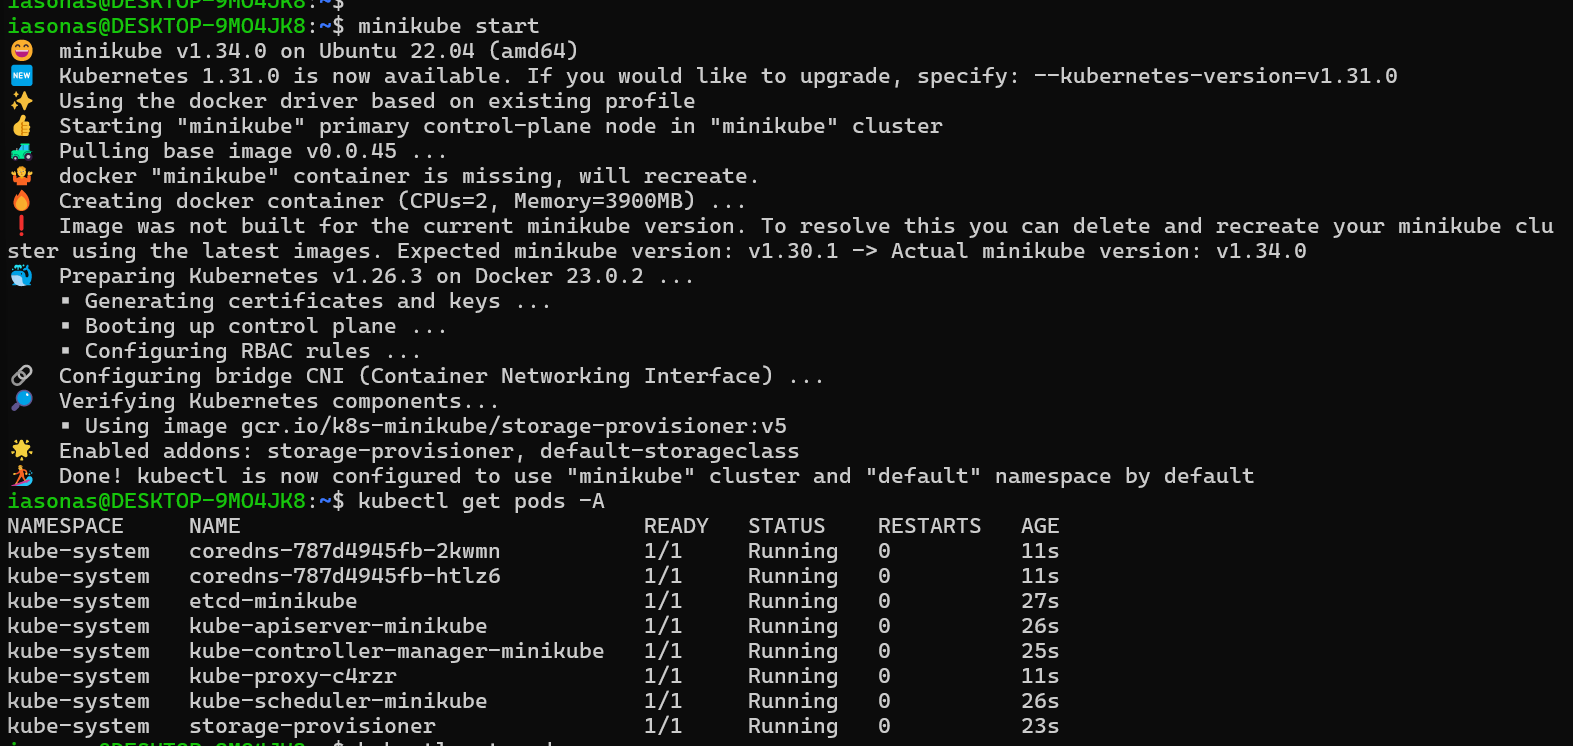
\includegraphics[width=1.5\textwidth]{graphics/minikube_deployment_k8s.png}
	\caption{\en{Minikube deployment}}
\end{figure}

\subsection{Δημιουργία \en{Kubernetes manifest files}}

Στο πλαίσιο της ανάπτυξης της εφαρμογής, χρησιμοποιήθηκε το 
\en{Kubernetes} για τη δημιουργία και διαχείριση ενός \en{pod} 
που φιλοξενεί την εφαρμογή \en{Django}. Το αρχείο διαμόρφωσης \en{YAML}
(\en{pod1.yml}) που δημιουργήθηκε, ακολουθεί τη βασική δομή του \en{Kubernetes}, 
ορίζοντας τον τύπο πόρου ως \en{Pod} και 
εκχωρώντας μεταδεδομένα όπως το όνομα \en{djangotestapp}. 
Στην ενότητα \en{spec}, ορίζεται ένα \en{container} 
το οποίο χρησιμοποιεί την εικόνα \en{iasonasi/djangotestapp:latest} 
και ακούει στη θύρα 8000, η οποία είναι η προεπιλεγμένη θύρα της 
εφαρμογής \en{Django}. Παρακάτω το \en{spec} του \en{yaml file.}(σχήμα 8.6)

\FloatBarrier

\begin{figure}[h]
	\centering
	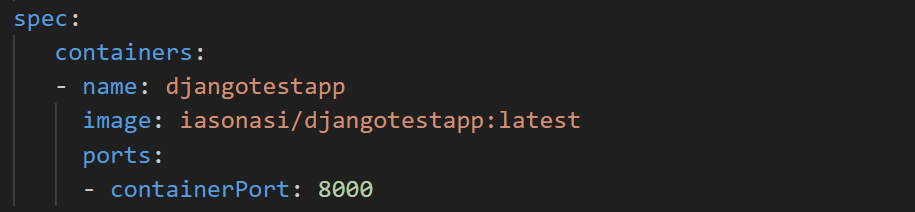
\includegraphics[width=1.5\textwidth]{graphics/pod_spec.png}
	\caption{\en{Spec}}
\end{figure}

\FloatBarrier

Αυτό το παράδειγμα αποδεικνύει τη σημασία της χρήσης του \en{Kubernetes YAML syntax} 
για την αυτοματοποιημένη ανάπτυξη και διαχείριση \en{containerized} 
εφαρμογών. Μέσω αυτής της διαδικασίας, η εφαρμογή μπορεί να 
επεκταθεί εύκολα σε διάφορα περιβάλλοντα και να κλιμακωθεί 
ανάλογα με τις ανάγκες. Το συγκεκριμένο αρχείο \en{YAML} 
επιτρέπει στο \en{Kubernetes} να εκτελέσει και να διαχειριστεί το 
\en{pod} με τρόπο ανεξάρτητο από το υποκείμενο σύστημα, 
εξασφαλίζοντας επαναληψιμότητα και δυνατότητα μεταφοράς του 
συστήματος σε διαφορετικές υποδομές. Στην παρακάτω εικόνα φαίνεται το 
\en{YAML file} που χρησιμοποιήθηκε(σχήμα 8.7). 

\FloatBarrier

\begin{figure}[h]
	\centering
	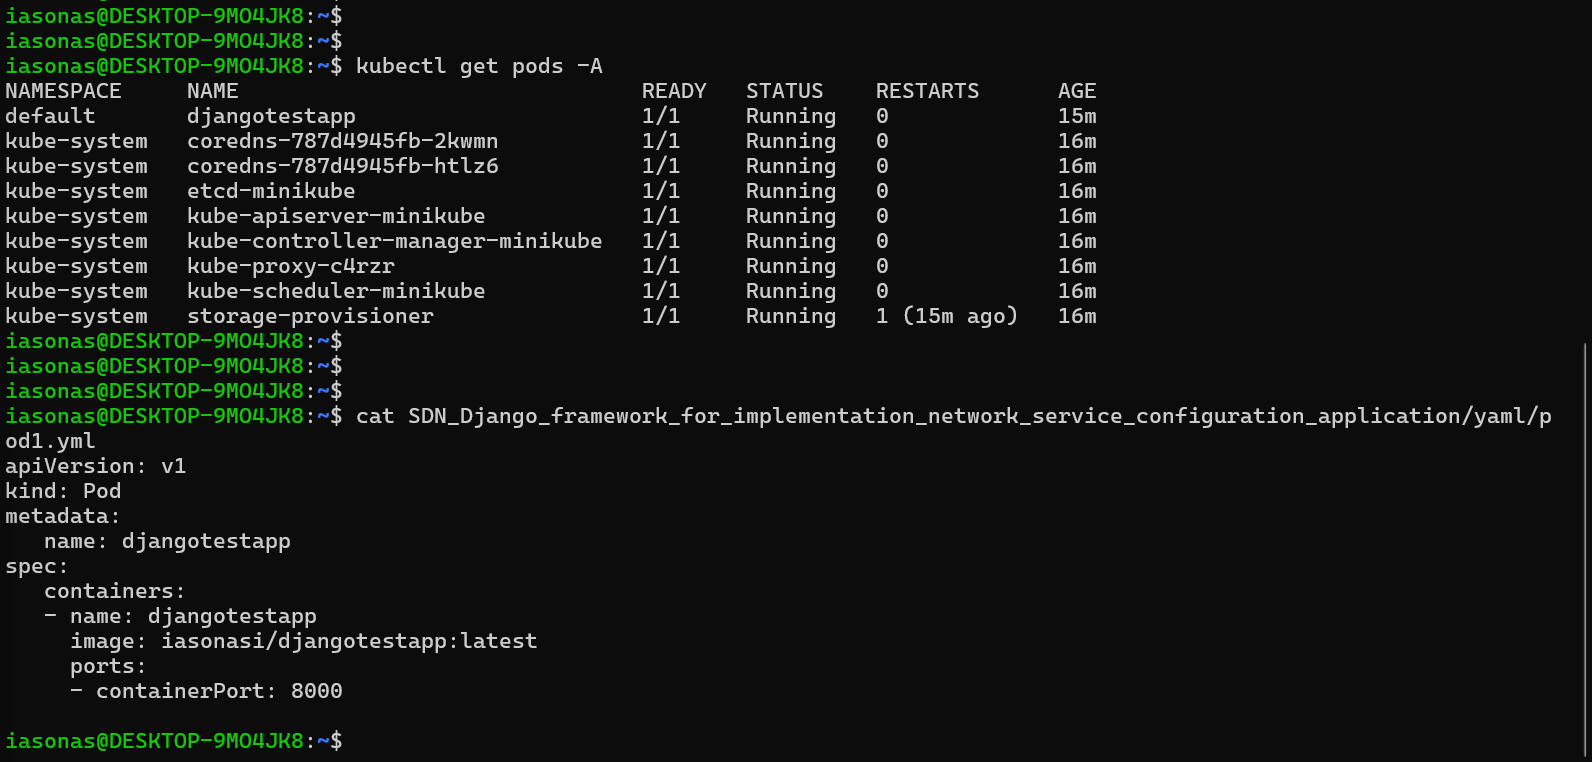
\includegraphics[width=1.5\textwidth]{graphics/deploy_django.png}
	\caption{\en{Manifest for Django pod}}
\end{figure}

\FloatBarrier

\subsection{Πρόσβαση στο \en{Django pod}}.

Για να αποκτήσουμε πρόσβαση στην εφαρμογή \en{Django} που τρέχει στο \en{pod} του \en{Kubernetes}, 
μπορούμε να χρησιμοποιήσουμε την εντολή \en{kubectl port-forward pod/djangotestapp 8000:8000}. Με την εντολή \en{kubectl port-forward} θα μπορέσουμε μέσα απο έναν \en{browser}
να έχουμε πρόσβαση στην εφαρμογή.

\FloatBarrier

\begin{figure}[h]
	\centering
	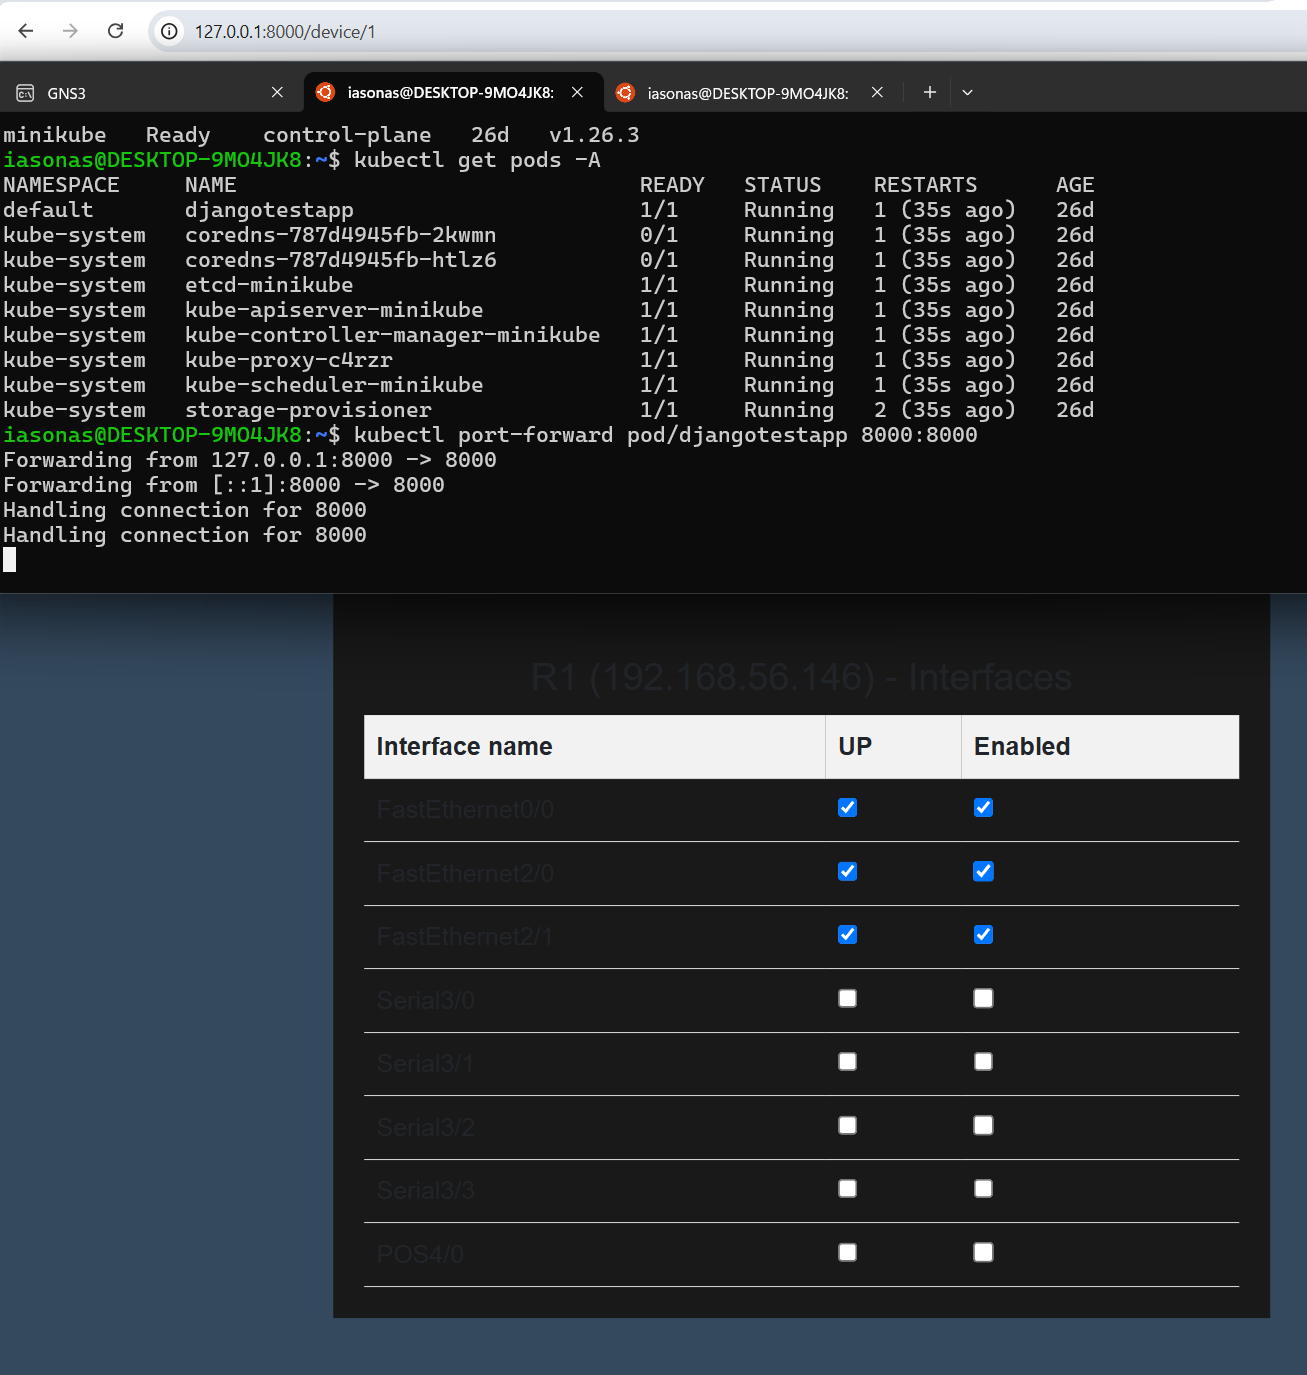
\includegraphics[width=1.5\textwidth]{graphics/kubernetes_proxy.png}
	\caption{\en{Port forward traffic}}
\end{figure}

\FloatBarrier

\noindent  Στη συνέχεια, επισκεφτείτε την εφαρμογή σας στον \en{browser} μέσω της διεύθυνσης \en{http://localhost:8000}. Θα πρέπει όλες οι λειτουργίες
να μπορούν να εκτελεστούν κάτι το οποίο η παραπάνω εικόνα το αποδεικνύει. 


\section{\en{Use cases} με \en{Kubernetes}}

Η ανάπτυξη μιας εφαρμογής σε περιβάλλον Kubernetes στοχεύει στη μετατροπή της σε μικροϋπηρεσία, προσφέροντας σημαντικά πλεονεκτήματα. Αυτή η αρχιτεκτονική διευκολύνει την κλιμάκωση μέσω των μηχανισμών του Kubernetes, όπως το \en{Horizontal Pod Autoscaler} (\en{HPA}), το οποίο επιτρέπει την αυτόματη προσαρμογή των πόρων της εφαρμογής προσθέτοντας επιπλέον \en{replica}. Στο πλαίσιο της παρούσας διπλωματικής εργασίας, η υλοποίηση περιορίστηκε στη δημιουργία \en{pod}. Παρόλα αυτά, η μετατροπή της εφαρμογής σε μικροϋπηρεσία διευκολύνει την αξιοποίηση των δυνατοτήτων του Kubernetes, καθώς η ενσωμάτωση οποιουδήποτε αντικειμένου, όπως το \en{HPA}, πραγματοποιείται εύκολα μέσω της κατάλληλης διαμόρφωσης σε \en{YAML file}.

Η χρήση Kubernetes στη συγκεκριμένη εφαρμογή αποσκοπεί στην αύξηση της ευελιξίας και της προσαρμοστικότητάς της σε περιόδους υψηλής ζήτησης. Ενώ μια μονολιθική εφαρμογή παρουσιάζει περιορισμούς στην επέκταση, η αρχιτεκτονική μικροϋπηρεσιών επιτρέπει δυναμική κλιμάκωση, διασφαλίζοντας τη βέλτιστη λειτουργία της εφαρμογής σε κάθε συνθήκη.